\chapter{State of the art}
\label{chap:soa}

In this chapter we ....


\section{ABR Video Streaming}
\label{sec:abr}

There are three ways of media delivery over \textit{HTTP}. The first method is by
\textbf{file download}, the media file is entirely stored in a local hard drive and played afterwards.
The second method is called \textbf{progressive download}, in which the file is stored in a local 
hard drive but instead the download starts from the beginning and the media can be played when
enough data are available. However, these two methods have disadvantages like waste of bandwidth,
\textit{DRM} issues and also requiring a reliable transmission. The last method is called
\textbf{streaming}, contrary to the former two, the file is not stored locally, but played from
the server, the client needs a data buffer to store the data that is being downloaded and
when the session is closed the data are deleted.

Streaming media also comes with some challenges. There are a lot of network variability
and a big heterogeneity in video capable devices. Therefore, to solve these shortcomings,
\textit{Adaptive bitrate streaming (ABR)} was created.

The basic idea of \textit{Adaptive bitrate streaming} is to adapt the media content
for the user by monitoring different parameters like estimated bandwidth, buffer level or
\textit{CPU load}, see \autoref{fig:abrtime}. There are many propietary adaptive streaming solutions:

\begin{itemize}[topsep=0.5pt]
  \setlength\itemsep{0.5pt}
  \item \textbf{\textit{Apple HTTP Live Streaming (HLS)}}: \textit{HTTP Live Streaming HLS}
  is an implementation of an \textit{ABR} protocol over \textit{HTTP} developed by Apple \cite{hls1}
  as part of the QuickTime software and the mobile operating system \textit{iOS}. \textit{HLS} 
  supports live streaming and video on demand. \textit{HLS} is proposed in 2009 as a standard to
  the \textit{IETF} \cite{hls2}.
  \item \textbf{\textit{Microsoft Smooth Streaming (MSS)}}: \textit{Smooth Streaming} is part
  of \textit{Internet Information Services (IIS) Media Services} for delivering media over
  \textit{HTTP} \cite{mss1}. A prototype version of \textit{Smooth Streaming}
  was used to deliver live and on-demand streaming content from such events as the Summer Olympic
  Games in Beijing and the Democratic National Convention in Denver.
  \item \textbf{\textit{Adobe HTTP Dynamic Streaming (HDS)}}: \textit{HTTP Dynamic Streaming}
  is the implementation of adaptive streaming by Adobe. \textit{HDS} enables high-quality, network
  efficient HTTP streaming for media delivery that is tightly integrated with Adobe software \cite{hds1}. The
  solution is based in using \textit{Open Source Media Framework (OSMF)} and Adobe Flash Player.
\end{itemize}

\begin{figure}[h]
  \centering
  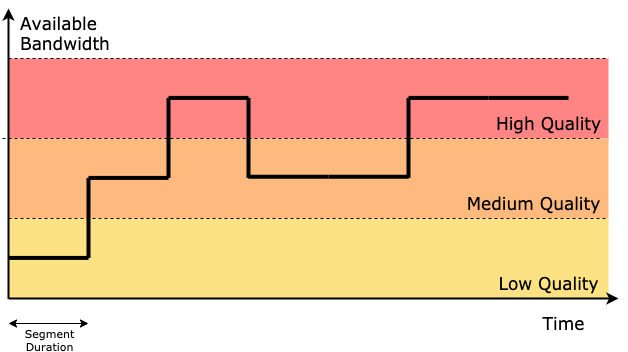
\includegraphics[width=0.7\textwidth]{img/abrtime.png}
  \caption{Evolution of segment quality with time}
  \label{fig:abrtime}

\end{figure}

But there was no official standarization for adaptive video delivery over HTTP. For that reason,
a new international stadard called \textit{MPEG-DASH} was developed and published.

\section{Dynamic Adaptive Streaming over HTTP}
\label{sec:dash}

The \textit{DASH} standard was created between the \textit{Moving Picture Experts Group} from \textit{ISO/IEC}
and the \textit{3GPP}. The development for \textit{DASH} started in January 2009 and completed in March 2010.
\textit{MPEG-DASH} was published in April 2012 but has been revised in 2019 as \textit{MPEG-DASH ISO/IEC 23009-1:2019}
\cite{ISO23009}. The \textit{3\textsuperscript{rd} Generation Partnership Project} defined the use of
\textit{DASH} as the standard of digital media delivery in mobile networks (3G GSM, 4G LTE) in \cite{3gpp1}.

The objective of \textit{DASH} was to create a unique standard that replaces the propietary solutions
from Microsoft, Apple and Adobe. Also, it will offer the interoperability and the convergence necessary for
the growth of big scale video streaming solutions. Microsoft, Apple, Netflix, Qualcomm,
Ericsson and Samsung also took part of the development of the standard.

One of the biggest advantages of \textit{DASH} is that the video streaming is over \textit{HTTP} version 1.1 protocol
(\textit{HTTP/1.1}). The use of \textit{HTTP} means that reusing existing internet infrastructure and
media content distribution tecniques using \textit{CDN (Content Delivery Networks)} can be done.
Another convenience of using \textit{DASH} is that due to using \textit{HTTP} encapsulation, problems
with passing through firewalls and the \textit{Network Address Translation (NAT)}
are not existent.

All the control of the media content delivery is located in the \textit{DASH} client side. The
standard does not define any web delivery mechanism nor the bitrate adaptation algorithm. What \textit{DASH}
does define in \cite{ISO23009} are:

\begin{itemize}
  \item \textit{\textbf{The Media Presentation Description (MPD) File Format}}: The \textit{MPD} file
  uses the \textit{eXtensible Markup Language (XML)} and
  contains the specifications of the media content and the \textit{URL} of the segments
  in the \textit{HTTP} video servers.
  \item \textbf{Segment format}: \textit{DASH} defines the characteristics of the necessary
  codifications and the way that the media content is divided in small fragments called 
  \textit{segments}.
\end{itemize}


\begin{figure}[h]
  \centering
  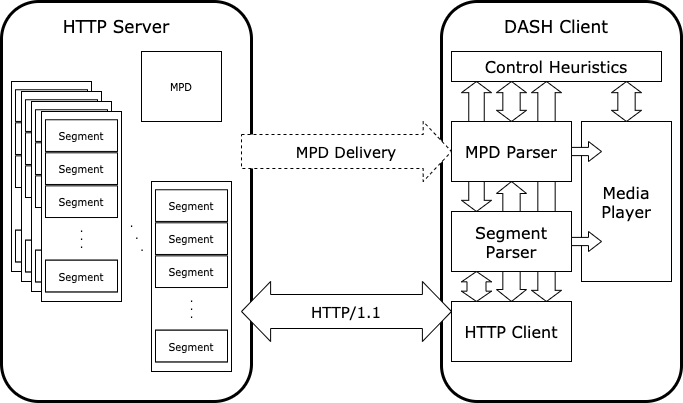
\includegraphics[width=0.7\textwidth]{img/dasharch.png}
  \caption{DASH client-server architecture. Source: MPEG \cite{ios1}}
  \label{fig:dasharch}
\end{figure}

The \autoref{fig:dasharch} presents a simple \textit{DASH} architecture. The video and audio
content are processed and stored on an \textit{HTTP} server. To access the content, the client
sends \textit{HTTP} requests to the server. But first, the client needs to download the 
\textit{MPD} file, normally through \textit{HTTP}. The client then does the
parsing of the \textit{MPD}, extract information such as the duration of a segment, media types or 
resolutions. Finally, the \textit{DASH} client chooses the adequate quality and starts the 
streaming of the content using \textit{HTTP GET} request to fetch the segments.

The \textit{DASH} client stores the segments in a buffer and consumes the content. It continues
to fetch new segments and by monitoring network variables it will decide which quality (higher
or lower bitrate) to request next to avoid problems like buffer underflow and maintain at 
least a set number of segments in the buffer.

\subsection{MPD}
\label{sec:mpd}
The \textit{MPD} file is an \textit{XML} document that describes the characteristics
of the different media components that composes the media content (e.g. video, audio, subtitles).

The structure of the \textit{MPD} is hierarchical as illustrated in \autoref{fig:mpd}. The media content is divided in a sequence of
\textbf{periods}, each period has a starting time and a duration. In a period, the set of encoded
versions of the media content is consistent, that is, the same bitrates, languages and so on.

\begin{figure}[h]
  \centering
  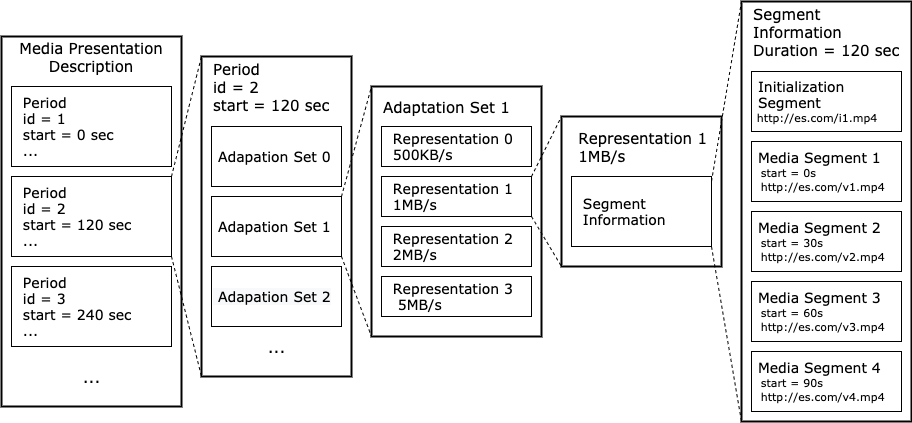
\includegraphics[width=\textwidth]{img/mpd.png}
  \caption{The MPD hierarchical data model. Source: MPEG \cite{ios1}}
  \label{fig:mpd}
\end{figure}

Each period consists of one or multiple \textbf{adaptation sets}. An adaptation set represents
an set of interchangeable encoded versions of one or serveral media content components. For instance,
and adaptation set may contain the different bitrates of the video component of the same multimedia content
and another adaptation set may contain the different bitrates of the audio component of the same multimedia
content.

An adaptation set contains a set of \textbf{representations}. A representation describe an enconded
alternative of the same media component, the alternatives can vary by bitrate, resolution, framerates, 
codec, sampling rate or other characteristics.

Each representation consists of one or multiple \textbf{segments}. A segment is the media stream chunks
in temporal sequence. Each segment has a \textit{URI}, the client will use this \textit{URI} to make
\textit{HTTP GET} requests to the video server. 


\subsection{Adaptation Algorithms}
\label{sec:adap}

////////

\subsection{QoS \& QoE Metrics}
\label{sec:qoemetrics}


The \textit{Quality of Service (QoS)} is defined by the \textit{ITU-T} in the document P.10/G.100
 \cite{itu2} as \textquotedbl The totality of characteristics of a telecommunications service that bear on its 
 ability to satisfy stated and implied needs of the user of the service\textquotedbl. And the \textit{Quality of 
Experience (QoE)} is defined as \textquotedbl The degree of delight or annoyance of the user of an application or service\textquotedbl.

The standard \textit{ISO/IEC 23009} defines a list of parameters for \textit{Quality of Service (QoS)} and
\textit{Quality of Experience (QoE)} for the adaptation algorithms to base on. There parameters 
is also used to evaluate the overall quality in the multimedia distribution service.

Some of the metrics are as follows:

\begin{itemize}
  \item \textbf{Average Throughtput}: This is a \textit{QoE} metric that defines a list in which 
  the average Throughtput observed in the client during a measuring period.
  \item \textbf{Initial Playout Delay}: This is a \textit{QoE} metric that represents the initial 
  delay in the reproduction of the media content.
  \item \textbf{Representation Switch Events}: This is a \textit{QoS} metric for measuring the 
  number of representation switch events of the multimedia content.
  \item \textbf{Buffer Level}: This is a \textit{QoS} metric that monitors the level of occupancy
  of the buffer during the reproduction of the multimedia content.
\end{itemize}


\section{Mobile Networks}
\label{sec:mobile}

The first mobile phone call was made in 1973 \cite{mob1}. New generations of mobile networks 
are developed almost every decade. The first generation 1G launched years later, but
it was only capable of doing voice calls. In 1991, the second generation 2G \textit{(GSM)} of 
mobile networks was introduced. \textit{GSM} provided improved wireless capabilities and 
introduced by the first time multimedia content with \textit{Multimedia Message Service (MMS)}.
But it was the third generation 3G, launched in 2001, that enabled new internet-driven
services such as video conferencing and streaming. Later in 2009, the \textit{LTE} 4G standard
was commercially deployed. With theorical download bandwidth of almost 100Mbps made high-quality
streaming into reality. 5G technologies improves in bandwidth even more and brings 
video streaming in \textit{UHD} and more.

The consumption of multimedia content on mobile networks is becoming increasingly relevant with 
the rise of bandwidth and ease of access. This section will provide a brief introduction to the 
basic concepts of mobile networks, their architecture and fundamentals.

\subsection{LTE}
\label{sec:4g}

\textit{Long Term Evolution (LTE)} was first introduced in 2008 in the Release 8 of the \textit{3GPP}
specification \cite{lte1}. The objective of \textit{LTE} was to migrate the \textit{3GPP} systems
into a optimized system based on packet switching (all \textit{IP}), with greater bitrates, lower
latency y multiple radio access technologies support.

\subsubsection{LTE Radio Interface}

\subsubsection{Architecture}
\label{sec:eps}

The design of the \textit{LTE} architecture was done from the ground up. The goal was to build a flat, all
\textit{IP} architecture using packet-switching, well structured (separation of control plane and user plane)
and with few elements.

\begin{figure}[h]
  \centering
  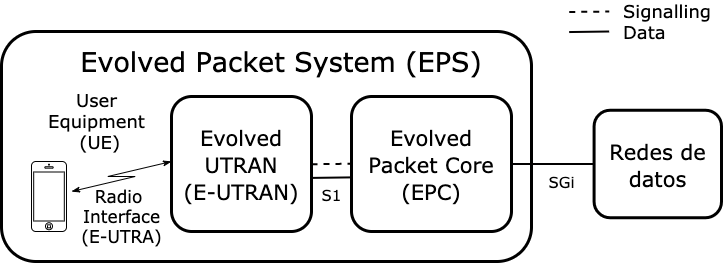
\includegraphics[width=0.8\textwidth]{img/eps.png}
  \caption{LTE Architecture}
  \label{fig:lte}
\end{figure}

The \textit{Evolved Packet System (EPS)} is constituted by the following elements:

\begin{itemize}
  \item \textbf{\textit{User Equipment (UE)}}: An \textit{UE} is any device used by an end user
  to communicate in a mobile network.
  \item \textbf{\textit{Evolved UMTS Terrestial Radio Access Network (E-UTRAN)}}: The only elements
  in the \textit{E-UTRAN} are the \textit{e-NodeB}. An \textit{\textbf{enhanced Node B (e-NodeB)}} works as a base station
  and a controller.
  \item \textbf{\textit{Evolved Packet Core (EPC)}}: 
\end{itemize}

MIMO

LTE enb phy

UM buffer size

propagation loss model

Fading loss model

Earfcn

Resource blocks


antenna model

\subsection{5G}
\label{sec:5G}


\section{Network Simulator 3}
\label{sec:ns3}



REM

MIMO

LTE enb phy

UM buffer size

TCP new reno?

Lossmodel

Fading loss model

Earfcn


Building